% \section{Loop Invariant Computation and Code Motion}

\section{Loop}

In a CFG, not every cycle is a loop from an optimization perspective.


A loop is a set of CFG nodes S such that:
\begin{itemize}
    \item there exists a header node h in S that dominates all nodes in S.
    \begin{itemize}
        \item there exists a path of directed edges from h to any node in S.
        \item h is the only node in S with predecessors not in S.
    \end{itemize}
    \item from any node in S, there exists a path of directed edges to h.
\end{itemize}
A loop is a single entry, multiple exit region.

\subsection{Dominance}

In a CFG, node a dominates b if every path from the start node to b passes through a. Node a is a dominator of b. The dominance relation is a partial order.


Node a strictly dominates b if $a \neq b$ and a dominates b.




\subsection{Natural Loops}

The natural loop of the back edge is defined to be the smallest set of nodes that includes the back edge and has no predecessors outside the set except for the predecessor of the header. Natural loops are the loops for which we find optimizations.

\subsection{Reducible Flow Graphs}
A flow graph is reducible if every retreating edge in any DFST for that flow graph is a back edge.

\paragraph{Testing reducibility} Take any DFST for the flow graph, remove the back edges, and check that the result is acyclic.

\paragraph{Example: Nonreducible Graph}



\begin{figure}[h]
    \centering
    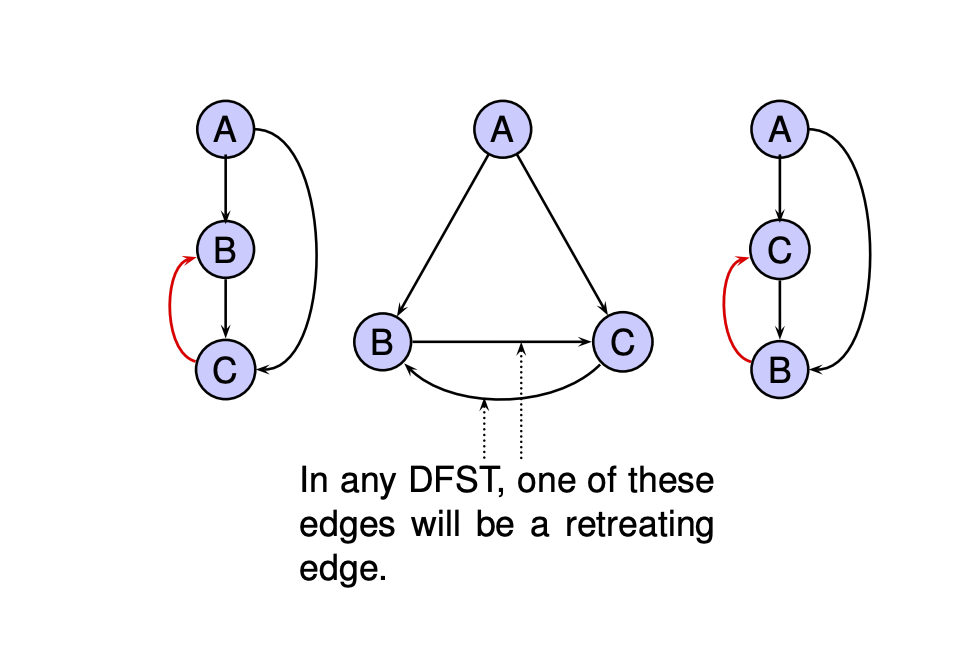
\includegraphics[width=0.5\textwidth]{images/DFST.png}
    \caption{Example: Nonreducible Graph }
    \label{fig:DFST}
\end{figure}

\subsection{Algorithm to Find Natural Loops}

\subsubsection{Step 1. Finding Dominators}

We can formulate this as Data Flow Analysis problem.
\begin{center}
 \begin{tabular}{|c|c|}
\hline Direction & Forward\\
\hline Values & Basic Blocks\\
\hline Meet operator & \( \cap \)\\
\hline Top(T) & Universal Set\\
\hline Bottom & $\phi$\\
\hline Boundary condition for entry node & $\phi$ \\  
\hline Initialization for internal nodes & \(\mathrm{T}\) \\
\hline Finited escending chain? &\checkmark  \\
\hline Transferfunction  & $\text { OUT }[\mathbf{b}]=\{\mathbf{b}\} \cup\left(\cap_{\{\boldsymbol{p}=\boldsymbol{p r e d}(\boldsymbol{b})\}} \text { OUT }[\mathbf{p}]\right)$ \\
\hline Monotone\&Distributive?  & \checkmark \\
\hline
\end{tabular}  
\end{center}



\subsubsection{Step 2. Finding Back Edges}

\paragraph{Depth-first spanning tree}
Edges traversed in a depth-first search of the flow graph form a depth-first spanning tree. We categorize edges in CFG as follows:
\begin{itemize}
    \item Forward edges (node to proper descendant).
    \item Retreating edges (node to ancestor).
    \item Cross edges (between two nodes, neither of which is an ancestor of the other.)
\end{itemize}

This is something difficult to understand. Let's make it simpler. We can number each node when we visit it. So each edge should be satisfied the following property:


\begin{center}
 \begin{tabular}{|c|c|}
\hline Forward edges  \( n_1 \rightarrow n_2\) & num($n_1$) $<$ num($n_2$) and  $n_1$ is ancestor of  $n_2$\\
\hline Cross edges  \( n_1 \rightarrow n_2\)& num($n_1$) $>$ num($n_2$) and neither  $n_1$ is ancestor of  $n_2$ nor $n_2$ is ancestor of  $n_1$ \\
\hline Retreating edges  \( n_1 \rightarrow n_2\) & num($n_1$) $>$ num($n_2$) and  $n_2$ is ancestor of  $n_1$\\
\hline
\end{tabular}  
\end{center}





Of these edges, only retreating edges go from high to low in DF order.

\paragraph{Back Edges}

A back edge \( t \rightarrow h \), h domiantes t.

\paragraph{Algorithm}

\begin{itemize}
    \item Perform a depth first search
    \item For each retreating edge \(t \rightarrow h\), check if h is in t’s dominator list
\end{itemize}

\subsubsection{Step 3. Constructing Natural Loops}

\paragraph{Algorithm} For each back edge $t\rightarrow h$:

\begin{itemize}
    \item delete h from the flow graph
    \item find those nodes that can reach t
(those nodes plus h form the natural loop of \(t \rightarrow h\))
\end{itemize}



\subsection{Inner Loops}





